We first evaluate the effectiveness of Roots as an anomaly detection mechanism. We experiment with
the SLO-based anomaly detector, using a simple HTML-producing web application called ``guestbook''.
This application allows users to login, and post comments. It uses the datastore service to save
the posted comments, and the user management service to handle authentication. We conduct all
of our experiments on a single node AppScale cloud except where specified. The node itself is an Ubuntu
14.04 VM with 4 virtual CPU cores (clocked at 2.4GHz) and 4GB of memory.

We run the SLO-based anomaly detector on guestbook with a sampling rate of 15 seconds, an analysis
rate of 60 seconds, and a window size of 1 hour. We set the minimum sample count to 100, and
run a series of experiments with different SLOs on the guestbook application. Specifically, we fix
the SLO probability at 95\%, and set the response time upper bound to $\mu + n\sigma$. 
$\mu$ and $\sigma$ stand for the mean and standard deviation of the
guestbook's response time, and these parameters are learned apriory by benchmarking
the application. We vary the value of $n$ between 2 and 5 in different experimental runs.

We also inject performance faults into AppScale by modifying its code. We run a set of experiments
by injecting faults into the datastore service. Our fault injection logic activates once every hour, and
slows down all datastore invocations by 45ms within a period of 3 minutes. 45ms is equal 
to $\mu + 5\sigma$. Therefore this delay causes all the SLOs in our experiments to get violated. 
We run a similar set of experiments where
we inject faults at the user management service of AppScale. Each experiment is run for a 
period of 10 hours.

\begin{table}
\begin{center}
\begin{tabular}{|c|p{1cm}|p{1cm}|p{1cm}|}
\hline
Faulty Service & $\mu + 2\sigma$ (31ms) & $\mu + 3\sigma$ (36ms) & $\mu + 5\sigma$ (45ms) \\ \hline
datastore & 18 & 11 & 10 \\ \hline
user management & 19 & 15 & 10 \\ \hline
\end{tabular}
\end{center}
\caption{Number of anomalies detected in guestbook app under different SLOs when
injecting faults into two different PaaS kernel services.
\label{tab:anomaly_counts}
}
\end{table}

Table~\ref{tab:anomaly_counts} shows how the number of anomalies detected by 
Roots in a 10 hour period varies when the SLO is changed. The number of anomalies
drops noticeably when the response time upper bound is increased. When the
SLO is set to $\mu + 5\sigma$ (45ms), the only anomalies detected are the ones
caused by our hourly fault injection mechanism. As the SLO is tightened by lowering the upper bound,
Roots detects additional anomalies. These additional anomalies
result from a combination of injected faults, and other naturally occurring faults
in the system.

\begin{figure}
\centering
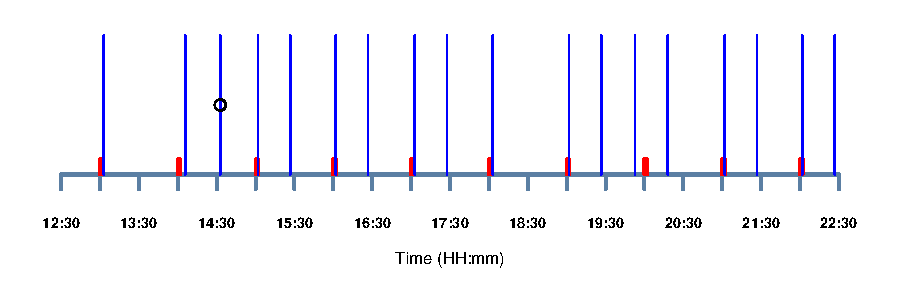
\includegraphics[scale=0.6]{time_line_guestbook_2s}
\caption{Anomaly detection in guestbook application (timeline).}
\label{fig:time_line_guestbook_2s}
\end{figure}

Next we analyze how fast and often Roots can detect anomalies in an application. We
first consider the case where we use $\mu + 2\sigma$ as the application SLO, and 
inject faults into the datastore service. Figure~\ref{fig:time_line_guestbook_2s} shows
anomalies detected in guestbook as events on a time line. The horizontal axis represents 
passage of time. The red markers indicate the time windows in which we injected faults into
AppScale. Each window is 3 minutes wide, and therefore appears thin in the full 10 hour scale
of the plot. The tall blue lines indicate the Roots anomaly detection events.
Note that every fault injection window is immediately followed by an anomaly
detection event, implying near real time reaction from Roots. The only exception is the fault
injection window at 20:00 hours which is not immediately followed by an anomaly 
detection event. Roots detected another naturally occurring anomaly at 19:52 hours
which caused the anomaly detector to go into the warm up mode. Therefore Roots
did not detect the faults injected at 20:00 hours. But as soon as the detector became
active again at 20:17, it detected the anomaly.